\documentclass[11pt]{article}
\usepackage{fullpage,amsmath,amssymb,amsthm,graphicx,enumerate,float}
\usepackage[english]{babel}
%\usepackage[ruled]{algorithm2e}

%%%%%%%%%% Start TeXmacs macros
\newcommand{\nocomma}{}
\newcommand{\tmem}[1]{{\em #1\/}}
\newenvironment{enumeratealpha}{\begin{enumerate}[a{\textup{)}}] }{\end{enumerate}}
\newenvironment{enumeratenumeric}{\begin{enumerate}[1.] }{\end{enumerate}}
\newenvironment{enumerateroman}{\begin{enumerate}[i.] }{\end{enumerate}}
\newenvironment{itemizedot}{\begin{itemize} \renewcommand{\labelitemi}{$\bullet$}\renewcommand{\labelitemii}{$\bullet$}\renewcommand{\labelitemiii}{$\bullet$}\renewcommand{\labelitemiv}{$\bullet$}}{\end{itemize}}
\newtheorem{lemma}{Lemma}
\newtheorem{theorem}{Theorem}
%%%%%%%%%% End TeXmacs macros

%%%%%%%%%% Begin Custom macros
\newtheorem{remark}{Remark}
\floatstyle{ruled}
\newfloat{algorithm}{thp}{lop}
\floatname{algorithm}{Algorithm}
\newcommand{\namedalgorithm}[2]{
    \begin{algorithm*}[t]
    \caption{#1}
    #2
    \end{algorithm*}
}

\newcommand{\OMIC}{\ensuremath{\mathsf{OMIC}}}
\newcommand{\OMC}{\ensuremath{\mathsf{OMC}}}
\newcommand{\SMIC}{\ensuremath{\mathsf{SMIC}}}
%%%%%%%%% End Custom Macros

\clubpenalty=10000 
\widowpenalty = 10000 

\begin{document}

\title{The Generalized Byzantine Model}

\author{
    Wang Cheng~\protect\footnote{\'{E}cole Polytechnique F\'{e}d\'{e}rale de Lausanne,Switzerland, cheng.wang@epfl.ch, +41 78 924 08 90.}
    \and
    Carole Delporte-Gallet~\protect\footnote{LIAFA-Universit\'{e} Paris-Diderot, Paris, France, cd@liafa.univ-paris-diderot.fr, +33 1 57 27 92 25.}
    \and
    Hugues Fauconnier~\protect\footnote{LIAFA-Universit\'{e} Paris-Diderot, Paris, France, hf@liafa.univ-paris-diderot.fr, +33 1 57 27 92 25.}
    \and
    Rachid Guerraoui~\protect\footnote{\'{E}cole Polytechnique F\'{e}d\'{e}rale de Lausanne, Switzerland, rachid.guerraoui@epfl.ch, +41 21 693 52 72.}
    \and
    Anne-Marie Kermarrec~\protect\footnote{INRIA Rennes Bretagne-Atlantique, France, anne-marie.kermarrec@inria.fr, +33 2 99 84 25 98.}
}

\maketitle

\begin{abstract}

The classical Byzantine model assumes that a process is either correct and obeys the protocol assigned to it, or is Byzantine and may  behave completely arbitrarily, sending corrupted messages to all processes during its entire execution. In this paper we generalize that model and consider a distributed model of computation where, in each communication step, some of the processes might send corrupted messages to a \tmem{subset} of the processes. We argue that this model enables to capture more accurately  practical situations where processes experiment bugs in specific parts of their code. We present this model and prove bounds on the number of correct processes needed to solve the classical interactive consistency and consensus problems.

\end{abstract}

\vspace{4cm}
\begin{center}
\Large This paper is a regular submission.\\
\Large The paper is a student paper.
\end{center}

\newpage
\pagenumbering{arabic}\setcounter{page}{1}

\section{Introduction}

Pease, Shostak and Lamport were the first to introduce
the Byzantine model in their landmark
paper~\cite{lamport1982byzantine,pease1980reaching}.
In their model, a Byzantine process is defined as a process that can
arbitrarily deviate from the protocol assigned to it.
They proved that  agreement is achievable
with a fully connected network if and only if the number of Byzantine
processes is less than one third of the total number of
processes. Dolev extended this
result to general networks, in which the connectivity number is twice
the number of faulty processes \cite{dolev1982byzantine}.
The early work on Byzantine agreement
is well summarized in the survey by Fisher~{\cite{fischer1983consensus}}.

Many approaches have been proposed to circumvent the impossibility results of
\cite{fischer1985impossibility} in the Byzantine context.
The work presented in \cite{dwork1988consensus} introduced the concept
of partial synchrony: an intermediate model between
synchronous and asynchronous models, allowing some
limited periods of asynchrony. Partial synchrony is considered weak enough to model  real systems
while  strong enough to make Byzantine agreement solvable.
% possible while being more practical compared to synchrony.
Alternative approaches rely on randomized algorithms (e.g.
{\cite{braud2013fast,dwork1988fault,king2011load,rabin1983randomized}}).

Accounting for the fact that communication failures sometimes dominate
computation ones (due to high reliability of hardware and operating systems), other models
focus on communication failures (e.g.
~{\cite{perry1986distributed,schmid2002formally}}) and hybrid failures
(e.g.~{\cite{gong1998byzantine,lincoln1993formally}}). Such models
consider that the Byzantine components are the communication channels instead of 
(in addition o) the processes.
For instance, in \cite{santoro1989time,santoro2007agreement}, Santoro and Widmayer
showed that consensus cannot be achieved with $\left[ \frac{n}{2} \right]$
Byzantine communication faults.
%
% There are models consider communication failures (e.g.
% {\cite{perry1986distributed,schmid2002formally}}) and hybrid failures
% (e.g. {\cite{gong1998byzantine,lincoln1993formally}}), since
% communication failures over computation are increasing important in modern
% distributed system due to high reliability of modern processes and robust
% operate system. When compared to component fault, the most significant feature
% of communication failures is dynamic. In the paper
% {\cite{santoro1989time,santoro2007agreement}}, Santoro and Widmayer
% showed that consensus cannot achieve with $\left[ \frac{n}{2} \right]$
% Byzantine communication faults.
% %Other round-based models have been studied by
%Charron-Bost and Schiper {\cite{charron2009heard}} (the heard-of model), and
%by Schimd et al. {\cite{biely2011synchronous}} (a comprehensive hybrid model).

% \subsection*{Motivation}
%In spite of many different models in the literature, the primitive failures
%they consider are Byzantine failure, communication failure and benign failure
%(e.g. omission failure, manifest failure, etc.).
In the classical Byzantine failure model, as well as in models with Byzantine communication channels, the notion of Byzantine failure is sustainable over time: the models consider that the processes (resp. the channels) are either Byzantine or are correct for the entire duration of the computation. More specifically, the Byzantine failure model encompasses two different situations: (1) A system attack where an adversary coordinates the behavior of several processes (resp. channels) in order to corrupt the system (e.g. denial of service attack); (2) Software or hardware bugs that lead one or several processes (resp. channels) to behave in an arbitrary manner.
We argue that
assumptions are fairly different in these two situations. Typically, under
attack, the set of Byzantine processes might indeed send corrupted messages systematically, possibly
with the sole purpose of corrupting the entire execution of the algorithm. In a situation where processes misbehave due to bugs, the number of corrupted messages might vary over time. Somehow, the Byzantine failure model as defined in \cite{lamport1982byzantine,pease1980reaching} is too conservative. It assumes the worst: failures occur due to a malicious intent rather than simply arbitrary bugs located in specific parts of the code.

In this paper we generalize the Byzantine failure model, accounting
for these differences and reconsider some of the theoretical impossibilities in
this light. We study our  \tmem{generalized Byzantine model} in a synchronous context
of $n$
processes of which up to $m$ can be faulty. The processes can
communicate with each other directly through a complete network.
We assume that each faulty process (partially controlled by
the adversary) is associated with up to $t$ Byzantine communication
links. We call such a process the
{\tmem{$t$-faulty process}}.
%AMK:so the processes are just faulty and channels are Byzantine right?
These $t$ Byzantine links are \tmem{dynamic}: they may be
different in different communication rounds.
Note that if $t=n$, our generalized Byzantine model instantiates the classical Byzantine model. From the component failure model's view, our generalization is orthogonal to those of \cite{tseng2013iterative} or \cite{santoro2007agreement}. When $m=t$, our model is a pure communication failure model. 
% Our model merges the advantages of the classical Byzantine model \cite{lamport1982byzantine} and the
 % communication failure model \cite{santoro2007agreement}, which enables it to tolerate $O(m t)$ 
% faulty links and to be dynamic meanwhile.


In this paper, we focus on the case when $t<n$.
The most important feature in this case is that {\tmem{$t$-faulty}}
processes always send correct messages to some processes in the system.
This enables us for instance to solve the \tmem{interactive consistency} problem~\cite{fischer1983consensus}.
%AMK: add ref

This problem consists in devising an algorithm
that allows every process $p$ to decide a value for each process $q$,
such that: (1) If $p$ and $q$ are correct, then $p$ decides the
initial value of $q$. (2) All correct processes decide the same
value for each process. Somehow, $t<n$ implies that the local
computation of the processes is always correct and only the
communication links related to the faulty processes are partially
controlled by the adversary - during specific rounds.
In this sense, we treat all the processes as
correct ones. In this context {\tmem{interactive consistency}}
means that every process knows the initial value of every other
process by the end of the computation.
% As a remark, in a system with
% all correct processes one can use {\tmem{interactive consistency}} to
% discover the transmission failures inside the system, for one can know
% the precise state and communication of the whole system.

The results obtained in the present paper are summarized in
Table~\ref{tab:results}. We give the necessary and sufficient
conditions for reaching interactive consistency with oral and signed
messages. Our sufficiency proofs are constructive and the algorithms
we provide are deterministic, while the necessity proofs are based on
scenario argument.
We also give a non-trivial upper bound for reaching \tmem{binary consensus} in Section \ref{sec:consensus}.


\begin{table}[h]
\centering
\begin{tabular}{|c|c|}
\hline
Oral messages & $n> \max \{ 2m+t,2t+m \}$\\
\hline
Signed messages & $n>2t+m$\\
\hline
\end{tabular}
\caption{\label{tab:results}Necessary and sufficient conditions for solving
interactive consistency with $t$-faulty failure.}
\end{table}

%!TEX root = synchrony.tex
\section{Model and definitions}
 
We consider a synchronous distributed system $P$ of $n$ processes. 
Each process is
identified by a unique id $p \in \{ 1, \ldots ,n \}$.  
As in {\cite{lamport1982byzantine,toueg1984simple}}, a
{\tmem{synchronous computation}} proceeds in a sequence of $rounds$.    
 The nodes communicate
with each other by sending messages round by round within a fully
connected 
point-to-point network.
In each round, every process first sends at most one message to every other process, possibly to all processes, 
and then $p$ receives the messages sent
by other  processes. The communication channels are authenticated,
that is to say the identity of the sender is known to the recipient. 

Each process has
an input register with its initial value from some domain $D$, and an
output register  
which records the outcome of the computation.
%The domain of input values 
Each process writes its output register at most once. When a
process writes its output register, we say that the process decides.
We model an algorithm as a set of deterministic automata, one for
every process in the system. 
Thus, the actions of a process are entirely determined by the
algorithm, the initial value and the messages it receives from others. 
In this paper we assume that processes always follow their protocol.


\vspace{1em}
\noindent{\bf Failures. }
In short, we consider a particular Byzantine model in which some faulty processes
may lie to others processes: even if the faulty process
follows its code, $p$ can send to some other processes Byzantine
messages, i.e. messages that result from $p$ not following the protocol.

More precisely, we assume an adaptive (or dynamic) adversary
which introduces Byzantine faults in transmission: these faults may
only come from faulty processes.

Here, up to $m$ of the
processes are 
faulty and controlled by the adversary. In each round, the adversary chooses
up to $t$ communication links from each faulty process that
will carry Byzantine messages. 


An instance of our model of $n$ processes with $m$ 
faulty processes such that in each round up to $t$ communication faults
on links from faulty processes may occur will be called an {\tmem{$( n,m,t )$-system}. In this paper, we always assume $m>0$, $t>0$, and $n \geqslant
max\{m,t\}$. We also assume $n>1$, the case $n=1$ being trivial. 

\vspace{1em}
 Concerning authentication of the communication, we consider two cases:
 \emph{oral messages} and \emph{signed messages}.
%  depending on the ability t
% We consider here the ability or not of authenticated messages with
% unforgeable signature~\cite{}
% Concerning Byzantine faults, an important  is the ability of having 
% the processes to send 
% unforgeable signed messages.
Following~\cite{lamport1982byzantine,srikanth1987optimal}, with oral messages, the
sender is always
authenticated by the receiver. But contrary to messages with
unforgeable signatures, a process $q$ may make process $p$ believe that it has received
message $m$ from process $r$ even if it is not true.
%Another important assumption is whether or not the model supports signatures. 
% We use oral messages and signed messages to model these two situations, 
% as in\cite{lamport1982byzantine,ST87}. An oral message is the one
% without signature. 
% and whose the  contents are completely controlled by the sender. 
For a signed message,  the sender attaches its
signature to the messages. 
A signed message satisfies the two following properties: 

\begin{enumeratealpha}
  \item A correct process's signature cannot be
    forged and any alteration of the content of its signed messages
    can be detected. 
  \item Any process can verify the authenticity of a process's
    signature. 
\end{enumeratealpha}
Note that the signature of a faulty process can be forged by
another faulty process. 

\vspace{1em}
\noindent{\bf Full information protocols.}
To prove our impossibility results, we consider full information protocol as in 
{\cite{fischer1982lower,lamport1982byzantine} or  in  the ``EIG''
  algorithm~\cite{lynch1996distributed}. In a full information
protocol, every process transmits to all processes in each round everything it knows
about all the values sent by other processes in the previous round.

We use $P^{l:k}$ to denote the set of strings of symbols in $P$ of length at least $l$ 
and at most $k$, $P^{+}$ to denote nonempty strings of symbols in $P$
and $P^{*}$ to denote all the strings including the empty one.

 A {\tmem{$k$-round scenario}} (for $(n,m,t)$-system $P$) describes an
 execution of the protocol. Intuitively  $\sigma$ describes a 
 communication scheme admissible for a $(n,k,m)$ system.
 It gives the initial value of each process and the communication scheme.
It captures the outcome of a $k$-round full information exchange.
Given scenario $\sigma$, 
$\sigma ( p_{1}
p_{2} \ldots p_{k} )$ is intended to represent the value $p_{k-1}$
tells $p_k$ that $p_{k-2}$ tells $p_{k-1}$ ... that $p_1$ tells $p_2$
is $p_1$'s initial value. 

 More formally,  a  {\tmem{$k$-round scenario}} $\sigma$
  is a mapping :$P^{1:k+1}
\rightarrow D$, such that:
\begin{itemize}
\item
For a string $p$ of length $1$, $\sigma(p)$ is $p$'s initial value. 
\item
There is a partition of $P$ into two sets $R_{\sigma} $, the set of
correct processes,  and $U_\sigma$, the set of faulty ones
such that:
\begin{itemize}
\item
$|U_\sigma| \leq m$ (and then $|R_\sigma|\geq n-m$)
\item
for every  process $p\in R_{\sigma} : \sigma(w p q) = \sigma(w p)$ for all
$q\in P$ and $w\in P^{0:k-1}$,  
\item
for every process $p\in U_\sigma$,  for every round $j$ in $\{1,\ldots
, k\}$,  there is a set $T$ of at most $t$ processes such that for
all $q\in P\setminus T$  and for all
$w\in P^{0:k-1}$ we have $\sigma(w p q) = \sigma(w p)$.
\end{itemize}
\end{itemize}
Note that if  $\sigma(wpq) \neq \sigma(wp)$ for some strings $w$ of
length $l$, that means that $q$  receives a Byzantine message from $p$
in round $l$.



If $\sigma$ is a
{\tmem{$k$-round scenario}} and $p \in P$, $p$'s view of \ $\sigma$ is
the map $\sigma_p$ defined by 
$\sigma_{p} ( w ) = \sigma ( w p )$. 


Let $O$ be the set of possible outputs and $\mathcal{U}^{k}$ be the
set of mappings from $P^{k}$ into $D$.
% A  $k$-round algorithm $\cal A$ defined in a $(n,m,t)$ system
% may be defined  on the set of all scenario; namely as a set $\{ F_{p}
% : p \in P \}$ of functions, 
% where $F_{p} : \mathcal{U}^{k}  \rightarrow O$. 
%  $\cal A$ solves a problem 
%  if for each $k$-round scenario $\sigma$ and every processes $p
% \in P$,  $F_{p} ( \sigma_{p} )$ satisfies the specification of the
% problem.
Any decision $k$-round algorithm $\cal A$ defined in an $(n,m,t)$ system
may be defined  on the set of all scenarios; namely as a set $\{ F_{p}
: p \in P \}$ of functions, 
where $F_{p} : \mathcal{U}^{k}  \rightarrow O$. 
Then without loss of generality, we consider in the following only algorithms
defined this way on the set of all scenarios by a set $\{ F_{p}
: p \in P \}$ of functions.

 $\cal A$ solves a problem 
 if for each $k$-round scenario $\sigma$ and every process $p
\in P$,  $F_{p} ( \sigma_{p} )$ satisfies the specification of the
problem.




\vspace{2em}
\noindent{\bf Problem specifications.}
We will first address the problem of {\tmem{interactive consistency}}~\cite{fischer1983consensus}. 
In this case, each process maintains an output register of $n$ entries. 
The $j$-th entry of the output register of a process $i$ contains the value decided by process $i$ for process $j$.
It is defined by the  two following properties:
\begin{itemizedot}
  \item {\tmem{Termination}}: Eventually, every process decides a value for
  each process.
  
  \item {\tmem{Validity}}: If process $p$ decides $v$ for process $q$, then
  $v$ should be the initial value of $q$.
\end{itemizedot}
As a remark, validity implies that all the processes decide the same
values.
Note that, contrary to classical models with faulty processes, here
even faulty processes have to decide. 

Let ${\cal A}= \{
F_{p} :p \in P \}$ be a $k$-round algorithm and the output is a vector that contains the  $n$ decided values then  $O$ is $(D\cup \{\bot\})^n$.
Then $\cal A$ solves  interactive
consistency if for each $k$-round scenario $\sigma$ and 
every process $p
\in P$,  $F_{p} ( \sigma_{p} )$ satisfies the Termination and Validity properties of interactive consistency, i.e.
for each $k$-round scenario $\sigma$ and all $p,r
\in P$ we have $F_{p} ( \sigma_{p} )[r] = \sigma ( r )$.


\vspace{1em}
We will also consider the {\tmem{binary consensus}} problem~\ref{fischer1983consensus}. 
In this problem, we assume that every process's input value is in $\{0,1\}$
and its output register contains $\bot$, 0 or 1. $\bot$ means that the
register has not yet written by the process. 
The value written in the output register is named the decision value.
The  {\tmem{binary consensus}} problem is defined by the three
following properties: 
\begin{itemizedot}
  \item {\tmem{Termination}}: Eventually, every process decides a value.
  \item {\tmem{Agreement}}: Every two processes decide the same value.
  \item {\tmem{Validity}}: If  all processes start with the same
    initial input, then every process should decide this value. 
\end{itemizedot}


Let ${\cal A}= \{
F_{p} :p \in P \}$ be a $k$-round algorithm and the output is in $\{0,1,\bot\}$.
Then $\cal A$ solves  binary consensus if for each $k$-round scenario $\sigma$ and 
every process $p
\in P$,  $F_{p} ( \sigma_{p} )$ satisfies the Termination, Agreement
and Validity properties of binary consensus, i.e.   
if for each $k$-round scenario $\sigma$, there exists $v$ the initial
value of some process such that  
for all processes $p$ and $r$,  we have $F_{p} ( \sigma_{p} ) = v$,
where $v$ is the initial value of some process.

%%% Local Variables: 
%%% mode: latex
%%% TeX-master: "synchrony"
%%% End: 


%!TEX root = synchrony.tex
\section{Interactive Consistency With Oral Messages}\label{oralIC}
In this section, we establish the tight bound for an $( n,m,t )$-system to
solve \tmem{interactive consistency} with {\tmem{oral messages}}. 

\begin{theorem}
  \label{consensusOral} It is possible to achieve  interactive consistency
  in an $( n,m,t )$-system with oral messages  if and only if $n> \max \{ 2m+t,2t+m \}$.
\end{theorem}

The proof of the theorem contains two parts with a series of lemmas. First, we
devise an algorithm we call OMIC to show the sufficiency of the theorem.
And then we show the necessary part based on scenario argument.

\subsection{Algorithm}
{\namedalgorithm{OMIC}{OMIC($0$):
\begin{enumeratenumeric}
%  \item Every process, suppose to be $i$, broadcasts its initial value, and denote the received value sent from $j$ as $v_j^i$. Let $v_i^i$ be the initial value of $i$.
    \item Every process  broadcasts its initial value.
    \item Every process receives the messages of the round.
      Let $v_j^i$ be the value received by $i$ from $j$, $v_i^i$ is the initial value of  $i$.
  %\item Set $ [ v_1^i, \ldots,  v_n^i ]$ as the output of process $i$
  \item Process $i$ decides $v_j^i$ as the initial value of process $j$
\end{enumeratenumeric}
OMIC($k$), $k>0$:
\begin{enumeratenumeric}
  \item Each process acts as a transmitter and sends its value to other
  $n-1$ processes (receivers).
  
  \item Every receiver process uses the value it gets in step $1$ as initial
  value, and executes OMIC($k-1$).
  %for one time to get the value other
  %receivers get in step $1$.
  
  \item After running algorithm OMIC($k-1$) in step 2, every receiver
  process get a vector of values representing what other receivers get from the
  transmitter, and then uses the majority values as its decision on the initial
  value of the transmitter process.
\end{enumeratenumeric}}}

Just like in
{\cite{lamport1982byzantine}}, we will use \tmem{transmitter} to denote the process
that wants to transmit its value, and use \tmem{receiver} to denote the process that wants to know the value of the transmitter. 

We first show the correctness of a special case of the algorithm, and then 
we show the general case by induction.
The considered special case is interesting because it shows that generally, we can get interactive consistency in two rounds.
More precisely, we show that in an $( n,m,t)$-system, two rounds are enough to achieve interactive consistency as soon as 
$n \geqslant 2 ( m+t )$.
Additional rounds are necessary only when the number of processes is between $2 ( m+t ) - 1$ and $ \max \{ 2m+t,2t+m \}$. Beyond that, Interactive consistency cannot be achieved.


\begin{lemma} \label{basicCase}
  \label{2roundlemma} If $n \geqslant 2 ( m+t )$, then the protocol OMIC($1$) achieves
  interactive consistency in $2$ rounds.
\end{lemma}

\begin{proof}
  Let us fix a process $p$ as a transmitter. If we prove that  each process decides  the
  initial value of $p$, then the lemma is proved.
  
  First suppose $p$ is correct, then all the receivers in the
  first round will get the initial value of $p$. In the second
  round when applying OMIC($0$), every receiver gets at most $m$ wrong
  values for $p$ due to the $m$ faulty processes.
As $n-1>2m$, each
  receiver decides the correct initial value of the transmitter.
  
  If $p$ is faulty, up to $t$ receivers will get wrong messages
  in the first round. Then in the second round, running OMIC($0$), every
  receiver gets at most $t+m-1$ wrong initial values for $p$,
  $m-1$ from the other faulty processes and $t$ from the receivers that have received wrong messages.
   Since $n>2 (t+m)$, $n-(t+m-1) > (t-m+1)$, the receiver receives a majority of the correct value and decides correctly.
\end{proof}

We now consider the case where additional rounds are necessary to achieve interactive consistency.

\begin{lemma} \label{reliableCorretness}
  \label{reliablecase}
  For any $k \geqslant 1$, if $n>2m+k$, if the transmitter is correct
 then every receiver in  OMIC($k$) decides on the initial value of the transmitter.
\end{lemma}

\begin{proof}
  The proof is by induction on $k$. Suppose the transmitter is correct. The
  lemma is trivial for $k=1$.
In the first round, all receivers get the initial value of the transmitter. In the second
  round when applying OMIC($0$), every receiver gets at most $m$ wrong
  values for $p$ due to the $m$ faulty processes.
 As $n-1>2m$, each
  receiver decides the correct initial value of the transmitter.

  We assume now the
  lemma is true for $k-1$ ($k>0$), and prove it for $k$.
  
%  Assume  that $n>2m+k$, then $n>2m+(k-1)$.
%  By induction hypothesis,  if the transmitter is correct
% then every receiver in  OMIC($k-1$) decides on the initial value of the transmitter.
 

%Consider now OMIC($k$).
  In the first step of the algorithm, the correct transmitter sends its value
  to the other $n-1$ receivers among which up to $m$ are faulty. 
  These receivers act as transmitters in OMIC($k-1$). 
  By induction hypothesis, if a transmitter is correct, every receiver in OMOC($k-1$)
  decides on the initial value of the transmitter.
  Then each receiver in OMIC($k$)  gets at least $n-1-m$ copies of the
  initial value in Step $3$. Since there are only $m$ faulty processes,
  $n-1-m>m+k-1 \geqslant m$, a majority of the values obtained  in Step $3$
  are the initial values. That is to say every process obtains the initial
  value of every correct process.
\end{proof}

\begin{lemma}
  \label{mainlemma}For any $k \geqslant 1$, OMIC($k$) ensures
  interactive consistency if $k \leqslant m$, $n>\min(2m+k,2m+2t-k)$.
\end{lemma}

\begin{proof}
  The proof is also by induction on $k$. If $k=1$, the condition is equal to $n>2m+2t-1$.
  Therefore by Lemma \ref{2roundlemma}, the lemma is proved.
  Now suppose
  the lemma is correct for $k-1$. We prove it for $k$.
  
  We first assume the transmitter is correct. Since $n>2m+k$, by lemma
  \ref{reliablecase} OMIC($k$) guarantees each process decides on  the initial
  value of the transmitter. So we have to verify the case in which
  the transmitter is faulty.
  
  If the transmitter is faulty, then at most $m-1$ of the receivers are
  faulty. Since $k-1<m-1$, $n-1>2m+ ( k-1 )$, and $n-1>2 ( m-1 ) +2t- (
  k-1 )$, OMIC($k-1$) ensures interactive consistency by induction hypothesis.
  Every receiver  knows the values that other receivers received in Step 1. As
  $n-1>2m+2t-k-1 \geqslant 2t$, the majority of the values the transmitter
  sent is the initial value of the transmitter. So all the processes decide
  the same correct value.
\end{proof}



\begin{lemma}\label{algICO1}
  If $m \geqslant t$ and $n>2m+t$, it is possible to achieve interactive consistency in an $(n,m,t)$-system 
  in $t+1$ rounds.
\end{lemma}

\begin{proof}
  Since $m \geqslant t$ and $n>2m+t$, we have $n>2t+t$ and $n >2m+2t-t$. Take
  $k=t$, by Lemma \ref{mainlemma} above, OMIC($m$) ensures
  interactive consistency. 
\end{proof}

\begin{lemma}\label{algICO2}
  If $t \geqslant m$ and $n>2t+m$, it is possible to achieve interactive consistency in an $(n,m,t)$-system 
 in $m+1$ round.
\end{lemma}

\begin{proof}
  Since $t \geqslant m$ and $n>2t+m$, we have $n>2t+m$ and $n >2m+2t-m$. Take
  $k=m$, by lemma \ref{mainlemma} above, OMIC($t$) ensures
  interactive consistency.
\end{proof}

From the above two lemmas, it is easy to deduce the sufficient part of 
Theorem~\ref{consensusOral}. 
If $m \geqslant t$ we gets the result by Lemma~\ref{algICO1} and  if $m<t$ by Lemma~\ref{algICO2}.



\subsection{Impossibility}

Now let us turn our attention to the necessary property of the theorem. We study two cases: $m \geqslant t$
and $t \geqslant m$. For each case, we proceed by contradiction.
We construct two scenarios such that there is a set of processes for which these two scenarios are indistinguishable. 
In the first scenario they have to decide 0 for that set of processes, while in the second scenario they have to decide 1.






\begin{lemma}\label{imposs:1}
  If $m \geqslant t$ and $n \leqslant 2m+t$, it is impossible to achieve interactive consistency in an $(n,m,t)$-system with oral messages.
  \end{lemma}

Due to space limitations, the proof is moved to Appendix \ref{app:imposs:1}. Here we describe the intuition behind the proof.
  $P$ can be partitioned into three non-empty sets $A$, $B$, and $C$,
  with $| A | \leqslant m$, $| B | \leqslant m$, $| C | \leqslant t$. 
  
  We define two scenarios $\alpha$ and $\beta$.
  In $\alpha$, all processes have 0 as initial values.
  Processes in $B$ are faulty and send  to processes $C$ messages
  pretending that processes in $A$ have 1 as initial value.
  
  In $\beta$, processes in $A$ have 1 as initial value and all  others processes have 0 as initial value.
  Processes in $A$ are faulty and send to processes in $C$ messages 
  pretending that processes in $A$ have 0 as initial value (see Figure~\ref{sc1}).
  
  In the two scenarios, processes in $C$ get the same messages, but in the first scenario 
  they have to decide 0 for processes in $A$ and $1$ in the second scenario leading to a contradiction.


\begin{lemma}\label{imposs:2}
  If $t \geqslant m$ and $n \leqslant 2t+m$, it is impossible to achieve interactive consistency in an $(n,m,t)$-system with oral messages.\end{lemma}

The proof of this Lemma is similar to the above one. Duo to space limitations, it is moved to Appendix \ref{app:imposs:2}.

From the above two lemmas, it is easy to deduce the necessary property of 
Theorem~\ref{consensusOral}. 
If $m \geqslant t$ we get the result by Lemma~\ref{imposs:1} and  if $m<t$ by Lemma~\ref{imposs:2}.







%!TEX root = synchrony.tex

\section{Interactive Consistency With Signed Messages}\label{signedMessage}

In this section we present the tight bound for an $( n,m,d )$-system to
reach \tmem{interactive consistency} with \tmem{signed messages}. In this new setting,
we have the following main result:

\begin{theorem}
  \label{consensusSigned} It is possible to achieve  interactive consistency
  in an $( n,m,d )$-system with signed messages  if and only if $n> 2d+m$.
\end{theorem}

As in the previous section, we rely on $2$ steps to prove this result.  We provide an algorithm, resp. a counterexample,  to prove  the sufficient, resp. the necessary property. 

The algorithm, called SMIC, is simple  and terminates in 3 rounds.


\subsection{Algorithm}
In the algorithm, called SMIC, each process $i$ maintains a list $V_{j}$, containing the possible initial values of process $j$.
{\namedalgorithm{SMIC}{\begin{enumeratenumeric}
  \item Every process broadcasts its initial values to all other
  processes (with its signature).
  
  \item Every process broadcasts the messages received in step $1$ with its 
  signature to all processes.
  
  \item Every process broadcasts the messages received in step 2 with its 
  signature to all processes.
\end{enumeratenumeric}
After this, every process $i$ has received messages like $\sigma ( j k l i
)$. For every $j,k$, if $\{ \sigma ( j k l i )\}_l$ have the same value $v$ for
different $l$, then 
%$i$ thinks the value $\sigma ( j k )$ is $v$ and 
$i$ appends $v$ into $V_{j}$ as the value $k$ received from $j$. 
%After $i$ checked this for all $j,k$, 
$i$ decides  for $j$ the 
%
%the initial
%value of $j$ to be the 
majority value in $V_{j}$.}}

\begin{lemma}
  If $n>m+2d$, an  $(n,m,d)$-system can reach interactive consistency with signed
  messages.
\end{lemma}

\begin{proof}
  If $j$ is correct, all the values $\sigma ( j k l i )$ will be the
  initial value of $j$ since the signature of $j$ can not be forged. So all the entries in $V_j$ are set to $\sigma (j)$, and the majority of $V_{j}$ is still $v$.
  
  If $j$ is faulty, suppose the initial value is $v$, as $n>m+2d$ at least $d+1$
  correct processes $\{k_1,...,k_{d+1}\}$ will receive $\sigma( j  k_{s}) = \sigma(j)$ equal to $v$. Since $k_s$ is correct, $\{\sigma(j k_s l i)\}_l$ are all $v$. This
  will contribute to at least $d+1$ values $v$ in $V_{j}$. On the other
  hand, only when $\sigma ( j k )$ is different from
  $v$, $k$ can contribute different values in $V_{j}$, because every $\sigma(j k)$ is always correctly sent to a subset of correct processes. Since $j$ can send at
  most $d$ wrong values in the first broadcast, $V_{j}$ contains at most $d$
  different values from $v$, which leads the majority value of $V_{j}$ to be
  $v$.
\end{proof}

Therefore the sufficient part of Theorem~\ref{consensusSigned} is proved. Now let us move to the necessary part.

\subsection{Impossibility}

Note that the two scenarios that we used in the proof of Lemma~\ref{imposs:1}
are now impossible. The processes in set $B$ cannot send to processes in set $C$ a message 
where they pretend that the initial values of processes in set $A$ are not the initial value that processes in $A$ have sent.

\begin{lemma}\label{imposs:3}
  If $n \leqslant m+2d$, it is impossible to achieve interactive consistency in an $(n,m,d)$-system with signed messages.
\end{lemma}


The proof of this necessary property of Theorem~\ref{consensusSigned} is similar to that of Lemma \ref{imposs:1}. Duo to space limitation, it is moved to Appendix \ref{app:imposs:3}.


%!TEX root = synchrony.tex
\section{An Upper Bound For Consensus}\label{sec:consensus}

In this section, we establish an upper bound for binary consensus with oral messages. 
In binary consensus, processes do not need to agree on the initial value of each process. 
They only need to  agree on some value to reach agreement.
%So in our setting, binary consensus is easier than interactive consistency.

\begin{theorem} \label{thmConsensus}
Binary consensus can be solved in a  $(n,m,d)$-system with oral messages if  $n>2m+d$.
\end{theorem}

We give a new algorithm OMC which is slightly different from OMIC. OMC achieves binary consensus.
%The basic idea in OMC consists in adding a \tmem{feedback step} to inform the transmitter about the guessed value other processes agreed on. The agreement is also based on majority selection. When $n$ is only greater than $2m+d$ (not max$\{2m+d,2d+m\}$), the majority value in algorithm OMIC may be several different values.
%So we assume a selection function \tmem{Major} to fix such situations. 
%\tmem{Major} takes a list as input. 
%The requirement we make for this function is that it alway returns the majority value in the input list. 
%If there are several values with the same highest count in the input, \tmem{Major} will return one of them. 
%The function is deterministic. The same input list (the order of the elements can be different) leads to the same output. 
%Each process $i$ maintains a list $V_i$ to record the
%guessed values for all processes.


The basic idea in OMC consists in adding a \tmem{feedback step} to inform the transmitter about the guessed value from the other processes. 
The agreement is also based on majority selection. 
%%%EXPLAIN
When $n$ is (only) greater than $2m+d$ (not max$\{2m+d,2d+m\}$), there could be several values 
with the same (most) counts in the selection of majority.
%%%
So we assume a deterministic function \tmem{Major} to fix such situations. 
\tmem{Major} takes a list as input. 
We require that this function  always returns the majority value in the input list. 
If there are several values with the same highest count in the input, \tmem{Major}  returns one of them. 
Each process $i$ maintains a list $V_i$ to record the
guessed values from each process.


{\namedalgorithm{OMC}{OMC($0$):
\begin{enumeratenumeric}
  \item Every process broadcasts its initial value in round $1$. Suppose process $i$ gets value $v_j^i$ (equal to $\varnothing$ if it receives nothing) from process $j$.
  
 % \item Every process, for example $i$ uses the value it receives from process $j(\neq i)$ as
 %$v_{j}$, or uses $\varnothing$ if it receives nothing. Let $v_i$ denote the initial value of $i$. 
 %Let $v_i$ denote the initial value of $i$. 
    \item 
  Processes $i$ takes $Major([ v_{1}^i ,\ldots ,v_{n}^i ])$ as output.

\end{enumeratenumeric}

OMC($k$), $k>0$:
\begin{enumeratenumeric}
  \item Each process acts as a transmitter and sends its value to other
  $n-1$ processes (receivers).
  \item Every receiver process uses the value it gets in Step $1$ as initial
  value, and executes OMC($k-1$) for one time to decide a value as a guessed initial value for the transmitter. 
  After this, receiver $i$ appends the guessed values into $V_i$. Note that there are $n-1$ transmitters different from $i$, so $V_i$ now has $n-1$ values.
  \item \tmem{Feedback step}:
  every receiver $i$ sends its guessed initial value for transmitter $j$ to $j$. $j$ adds the majority of the received values in this round into $V_i$ as the replacement of its initial value.
  \item Process $i$ takes $Major(V_i)$ as its output.
\end{enumeratenumeric}}}

As we already showed in Section \ref{oralIC}, if $n>2m+d$ we cannot guarantee interactive consistency with OMIC. 
However we ensure an interesting property in OMC for $n>2m+d$. 
More specifically,  we can prove that the elements in list $V_i$ are the same for different $i$, but the values in $V_i$ are not always equal to the initial values of the transmitters. 
We show this by induction as in Section \ref{oralIC}. Due to space limitation, the proof is moved to Appendix.

\iffalse
\begin{lemma}\label{cons:2}
If $n\geqslant 2m+2d$, then  OMC(1) achieves  binary consensus in $2$ rounds in a $(n,m,d)$-system.
\end{lemma}

\begin{proof}
As we have shown in Lemma~\ref{basicCase}, the guessed value in Step $2$ 
is the same as the initial value of transmitter when $n \geqslant 2m+2d$. 
As the output of each process is the result of applying \tmem{Major} to the list consisting of the initial values the properties of binary  consensus are satisfied.
\end{proof}

\begin{lemma}
For any $k\geqslant 1$, if $n>2m+k$, OMC($k$) ensures that the guessed value in Step $2$ for a correct transmitter is the initial value of the transmitter.
\end{lemma}

\begin{proof}
In the case $k=1$, the guessed value is the output of OMC(0) and  it is equal to the initial value of the correct transmitter since $n-1>2m$. Suppose the lemma is proved for $k-1$. Let us prove it for $k$.

In OMC($k$), the correct transmitter $i$ first sends its value to the other $n-1$ receivers. 
By induction hypothesis, the initial value of correct process will be guessed  correctly in OMC($k-1$). 
Since there are at least $n-1-m(>m)$ correct receivers, the decision values of all the receivers are the initial value of the transmitter.
\end{proof}

\begin{lemma}\label{cons:corelemma}
  For any $k \geqslant 1$, OMC($k$) achieves binary consensus if $n>\max\{2m+k,2m+2d-k\}$.
\end{lemma}

Note that this lemma is different from Lemma~\ref{mainlemma} because $k\leqslant m$ is not required.

\begin{proof}
We proof this lemma by induction on $k$. The basic case $k=1$ is the same as in Lemma~\ref{cons:2}.
Hence, we suppose the lemma is proved for $k-1$, and we prove it for $k$.

If the transmitter is correct, every receiver decides the same guessed value in Step $2$ for $n>2m+d$. 
If the transmitter is faulty, then
by induction hypothesis, every receiver  guesses the same value for every transmitter. 
In the \tmem{feedback step}, the transmitter will receive $n-1$ copies of the guessed value. 
Since there are at most $m$ faulty receivers, and $n-1>2m$, the transmitter 
also gets the same guessed value in Step $3$. 
So the final list $V_i$ is the same for different $i$ proving the agreement property. 

Now we consider  the validity property.
Suppose all input values are the same $v(\in \{0,1\})$. 
Since $n>2m+k$, by the last lemma, the guessed value for correct transmitters is the real initial value $v$. So there are at least $n-m (> m)$ elements in $V_i$ with value $v$. Therefore, \tmem{Major}($V_i$) is $v$. 
The validity property is also proved.
\end{proof}

With this core lemma, it is easy to prove Theorem~\ref{thmConsensus}.
\begin{proof}{(Proof of Theorem~\ref{thmConsensus})}
We prove the theorem by taking $k$ equal to $d$ in Lemma~\ref{cons:corelemma}.
\end{proof}
\fi

\begin{remark}
Though we have proved an upper bound for consensus, we know that this bound is not tight. 
For example, binary consensus is achievable with $m=1$ and $n=2m+d$. 
However, we conjecture that $2m+d$ is the tight bound if $m \geqslant n/3$.
\end{remark}
%%% Local Variables: 
%%% mode: latex
%%% TeX-master: synchrony
%%% End: 


%!TEX root = synchrony.tex

\section{Concluding Remarks}

In this paper, we introduced and investigated a generalized Byzantine model inspired by component and dynamic failures. We first considered the interactive consistency problem in this model, for which we gave necessary and sufficient conditions with oral and signed messages. We also provided an upper bound for reaching binary consensus. Then we explored a hybrid failure model which also covers crash failures.
Studying other problems in this model or applying it to the eventually synchronous 
context are interesting research directions. 

%Future work could focus on the consensus problem, partial synchrony or even asynchrony.
%Another possible thing one could do is to apply the methods in this paper to
%other models, especially for link failure models.

%%% Local Variables: 
%%% mode: latex
%%% TeX-master: synchrony
%%% End: 


\newpage

\bibliographystyle{abbrv}
\bibliography{ref}

\newpage
\appendix
%!TEX root = synchrony.tex

\section{Omitted Proofs}

\subsection{Proof of Lemma \ref{imposs:1}} \label{app:imposs:1}
\begin{proof}
\begin{figure}[h]
  \centering
  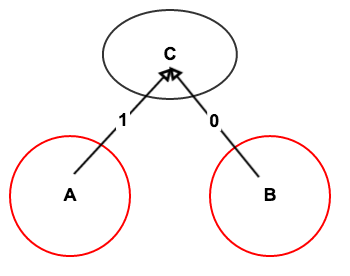
\includegraphics[scale=0.35]{impossible1.png}
  \caption{Case $m \geqslant d$  }
\end{figure}\label{sc1}

  The case $n=2$ is trivial. We assume $n \geqslant 3$.
  Suppose that $F$ is a $k$-round interactive consistency algorithm. Since $n \leqslant
  2m+d$, $P$ can be partitioned into three nonempty sets $A$, $B$, and $C$,
  with $| A | \leqslant m$, $| B | \leqslant m$, $| C | \leqslant d$. 
  
  We define two scenarios $\alpha$ and $\beta$.
  In $\alpha$, all processes have 0 as initial values.
  Processes in $B$ are faulty and send  to $C$ processes messages
  pretending that processes in $A$ have 1 as initial value.
  
   In $\beta$, processes in $A$ have 1 as initial value and all  others processes have 0 as initial value.
  Processes in $A$ are faulty and send to $C$ messages 
  pretending that processes in $A$ have 0 as initial value (see Figure~\ref{sc1}).
  
  In the two scenarios, processes in $C$ get the same messages, but in the first scenario 
  they have to decide 0 for processes in $A$ and $1$ in the second scenario leading to a contradiction.
    
More precisely  the scenarios $\alpha$
  and $\beta$ are defined as follows:
  \begin{enumerateroman}
    \item For every $w \in P^{+}$ not starting with a process of $A$, let
    \[ \alpha ( w ) = \beta ( w ) =0. \]
    \item For every $a \in A$, $b \in B$, $c \in C$ let
    \[ \alpha ( a ) = \alpha ( a a )  =  \alpha ( a b ) = \alpha ( a c )  = 0,
    \]
    \[ \beta ( a ) = \beta ( a a ) = \beta ( a b ) =1 \nocomma , \beta ( a c )
       =0. \]
    \item We define this part iteratively. 
    For every $a \in A$, $b \in B$, $c \in C$, $p \in P$, $w \in
    a P^{\ast}$, let
    \[ \alpha ( w c p ) = \alpha ( w c ) \nocomma , \alpha ( w a p ) = \alpha
       ( w a ) , \]
    \[ \beta ( w c p ) = \beta ( w c ) \nocomma , \beta ( w b p ) = \beta ( w
       b ) , \]
    \[ \alpha ( w b c ) = \beta ( w b ) \nocomma , \alpha ( w b a ) = \alpha
       ( w b ) , \]
    \[ \beta ( w a c ) = \alpha ( w a ) , \beta ( w a b )  =  \beta ( w a )
       . \]
  \end{enumerateroman}
  $\alpha$ is a  scenario in which processes in $B$ are faulty 
and  $\beta$ is a  scenario in which  faulty 
  processes are in set $A$. 
 Moreover,  $\alpha_{c} =
  \beta_{c}$ for all $c \in C$ then for any $a \in A$, $c \in C$
   \[ F_c ( \alpha_{c} )[a] = F_c ( \beta_{c} )[a].  \]

But for any $a \in A$, $c \in C$, as $F$ is a $k$-round  interactive consistency algorithm
    \[ F_c ( \alpha_{c})[a] = \alpha ( a ) = 0 , \] 
  \[ F_c ( \beta_{c} )[a] = \beta ( a ) =1 , \]
leading to a contradiction.
\end{proof}

\subsection{Proof of Lemma \ref{imposs:2}}\label{app:imposs:2}

\begin{proof}
\begin{figure}[h]
  \centering
  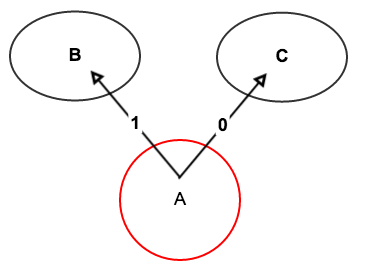
\includegraphics[scale=0.35]{impossible2.png}
  \caption{Case $d \geqslant m$  }
\end{figure}\label{sc2}

  This proof is similar to the proof above. 
  The case $n=2$ is trivial. We assume $n \geqslant 3$.
  Suppose that $F$ is a $k$-round  interactive
  consistency algorithm. Since $n \leqslant 2d+m$, $P$ can be partitioned into
  three non-empty sets $A$, $B$, and $C$, with $| A | \leqslant m$, $| B | \leqslant d$, $| C |
  \leqslant d$. 
  
   We define two scenarios $\alpha$ and $\beta$.
  In $\alpha$, all processes have 0 as initial values.
  Processes in $A$ are faulty and send to processes in $C$  messages
  pretending that they have  1 as initial value. 
  
   In $\beta$, processes in $A$ have 1 as initial value and all  others processes have 0 as initial value.
  Processes in $A$ are faulty and send to processes in $B$ messages 
  pretending that they have 1 as initial value (see Figure~\ref{sc1}).
  
  In the two scenarios, processes in $B$ and $C$  get the same messages, but in the first scenario 
  they have to decide 0 for processes in $A$ and $1$ in the second scenario giving the contradiction.
    
More precisely  the scenarios $\alpha$
  and $\beta$ are defined as follows:
  \begin{enumerateroman}
    \item For every $w \in P^{+}$ not starting with a process of $A$, let
    \[ \alpha ( w ) = \beta ( w ) =0. \]
    \item For every $a \in A$, $b \in B$, $c \in C$ let
    \[ \alpha ( a ) = \alpha ( a a )  =  \alpha ( a b ) =0, \alpha ( a c )  =
       1, \]
    \[ \beta ( a ) = \beta ( a a ) = \beta ( a c ) =1 \nocomma , \beta ( a b )
       =0. \]
    \item We define this part iteratively. For every $a \in A$, $b \in B$, $c \in C$, $p \in P$, $w \in
    a P^{\ast}$, let
    \[ \alpha ( w b p ) = \alpha ( w b ) , \alpha ( w c p ) = \alpha ( w c ) ,
    \]
    \[ \beta ( w b p ) = \beta ( w b ) \nocomma , \beta ( w c p ) =\beta ( w c ) ,
    \]
    \[ \alpha ( w a b ) = \alpha ( w a ) \nocomma , \beta ( w a c ) = \beta (
       w a ) , \]
    \[ \alpha ( w a c ) = \beta ( w a ) \nocomma , \beta ( w a b ) = \alpha
       ( w a ) . \]
  \end{enumerateroman}
 $\alpha$ and $\beta$ are scenarios in which processes in $A$ are faulty.
  Moreover, $\alpha_{b} =
  \beta_{b}$, $\alpha_{c} = \beta_{c}$ for all $b \in B$ and $c \in C$. 
  Then for any $a \in A$, $b \in B$:
   \[ F_b ( \alpha_{b} )[a] =F_b ( \beta_{b} )[a]. \]

  
But for any $a \in A$, $b \in B$, as $F$ is a $k$-round  interactive consistency algorithm
  \[ F_b ( \alpha_{b} )[a] = \alpha ( a )
     =0, \]
       \[ F_b ( \beta_{b} )[a] = \beta ( a )
     =1, \]
  leading to the contradiction.
\end{proof}

\subsection{Proof of Lemma \ref{imposs:3}} \label{app:imposs:3}

\begin{proof}
  Suppose that $F$ is a $k$-round  interactive consistency algorithm. 
  
  Since $n \leqslant
  m+2d$, $P$ can be partitioned into three nonempty sets $A$, $B$, and $C$,
  with $| A | \leqslant m$, $| B | \leqslant d$, $| C | \leqslant d$. 
  
   We define two scenarios $\alpha$ and $\beta$.
  In $\alpha$, all processes have 0 as initial values.
  Processes in $A$ are faulty and send  to processes in $C$  messages
  pretending that they have  1 as initial value. 
  
   In $\beta$, processes in $A$ have 1 as initial value and all  others processes have 0 as initial value.
  Processes in $A$ are faulty and send to processes in $B$ messages 
  pretending that they have 1 as initial value.
  

  
    In the two scenarios, processes in $B$ and $C$  get the same messages, but in the first scenario $\alpha$
  they have to decide 0 for processes in $A$ and $1$ in the second scenario giving the contradiction.
  
  We
  define scenarios $\alpha$ and $\beta$ as follows:
  \begin{enumerateroman}
    \item For every $w \in P^{+}$ not starting with a member of $A$, let
    \[ \alpha ( w ) = \beta ( w ) =0. \]
    \item For every $a_{1}  \in A^{+}$, $a \in A,b \in B,c
    \in C$, $w \in P^{\ast}$, let
    \[ \alpha ( a ) =0, \beta ( a ) =1, \]
    \[ \alpha ( a_{1}  b w ) = \beta ( a_{1}  b w ) =0, \]
    \[ \alpha ( a_{1}  c w ) = \beta ( a_{1}  c w ) =1. \]
    \item All other messages are sent and forwarded based on these messages
    correctly.
  \end{enumerateroman}
  
  $\alpha$ and $\beta$ are scenarios in which processes in $A$ are faulty.
  Moreover, $\alpha_{b} =
  \beta_{b}$, $\alpha_{c} = \beta_{c}$ for all $b \in B$ and $c \in C$. 
  Then for any $a \in A$, $b \in B$:
   \[ F_b ( \alpha_{b} )[a] =F_b ( \beta_{b} )[a]  \]

  
But for any $a \in A$, $b \in B$, as $F$ is a $k$-round  interactive consistency algorithm
  \[ F_b ( \alpha_{b} )[a] = \alpha ( a )
     =0, \]
       \[ F_b ( \beta_{b} )[a] = \beta ( a )
     =1, \]
  leading to a contradiction.
%  Note that, the only difference of $\alpha$ and $\beta$ is the initial value
%  of $A$. We can easy check that $A$ only lies to $B$ ($C$ resp.) for scenario
%  $\alpha$ ($\beta$ resp.). So it is impossible for $B$ or $C$ to tell the
%  real initial value of $A$ in these two scenarios.
\end{proof}

\subsection{Proof of Theorem \ref{thmConsensus}}

\begin{lemma}\label{cons:2}
If $n\geqslant 2m+2d$, then  OMC(1) achieves  binary consensus in $2$ rounds in an $(n,m,d)$-system.
\end{lemma}

\begin{proof}
As we have shown in Lemma~\ref{basicCase}, the guessed value in Step $2$ 
is the same as the initial value of transmitter when $n \geqslant 2m+2d$. 
As the output of each process is the result of applying \tmem{Major} to the list consisting of the initial values the properties of binary  consensus are satisfied.
\end{proof}

\begin{lemma}
For any $k\geqslant 1$, if $n>2m+k$, OMC($k$) ensures that the guessed value in Step $2$ for a correct transmitter is the initial value of the transmitter.
\end{lemma}

\begin{proof}
In the case $k=1$, the guessed value is the output of OMC(0) and  it is equal to the initial value of the correct transmitter since $n-1>2m$. Suppose the lemma is proved for $k-1$. Let us prove it for $k$.

In OMC($k$), the correct transmitter $i$ first sends its value to the other $n-1$ receivers. 
By induction hypothesis, the initial value of correct process will be guessed  correctly in OMC($k-1$). 
Since there are at least $n-1-m(>m)$ correct receivers, the decision values of all the receivers are the initial value of the transmitter.
\end{proof}

\begin{lemma}\label{cons:corelemma}
  For any $k \geqslant 1$, OMC($k$) achieves binary consensus if $n>\max\{2m+k,2m+2d-k\}$.
\end{lemma}

Note that this lemma is different from Lemma~\ref{mainlemma} in the sense that $k\leqslant m$ is not required.

\begin{proof}
We proof this lemma by induction on $k$. The basic case $k=1$ is the same as in Lemma~\ref{cons:2}.
Hence, we suppose the lemma is proved for $k-1$, and we prove it for $k$.

If the transmitter is correct, every receiver decides the same guessed value in step $2$ for $n>2m+d$. 
If the transmitter is faulty, then
by induction hypothesis, every receiver  guesses the same value for every transmitter. 
In the \tmem{feedback step}, the transmitter will receive $n-1$ copies of the guessed value. 
Since there are at most $m$ faulty receivers, and $n-1>2m$, the transmitter 
also gets the same guessed value in Step $3$. 
So the final list $V_i$ is the same for different $i$ proving the agreement property. 

Now we consider  the validity property.
Suppose all input values are the same $v(\in \{0,1\})$. 
Since $n>2m+k$, by the last lemma, the guessed value for correct transmitters is the real initial value $v$. So there are at least $n-m (> m)$ elements in $V_i$ with value $v$. Therefore, \tmem{Major}($V_i$) is $v$. 
The validity property is also proved.
\end{proof}

With this core lemma, it is easy to prove Theorem~\ref{thmConsensus}.
\begin{proof}{(Proof of Theorem~\ref{thmConsensus})}
We prove the theorem by taking $k$ equal to $d$ in Lemma~\ref{cons:corelemma}.
\end{proof}

\iffalse
\subsection{Proof of Theorem \ref{crashIC}}

\begin{lemma}
  If $n \geqslant 2 ( m+d )+c$, then the protocol OMIC'(1) achieves
  interactive consistency in 2 rounds.
\end{lemma}

\begin{proof}
  Suppose a transmitter $p$ with initial value $v ( v \neq \perp )$. The
  presence of crash-faulty processes can only send several copies of $v$ which
  contributes to several number of true value in majority selection, or
  several copies of $\perp$ which contributes nothing in majority selection
  since the number of $\perp$ is subtracted by $c$. So if $p$ does not crash,
  in step $3$ of OMIC'(1), the majority value is still $v$. If $p$ crashes in
  the first round, the value receivers get in step $2$ of OMIC'($1$) is
  $\perp$. Then in step $3$ every receiver gets at most $m$ values not equal
  to $\perp$, which makes the majority values to be $\perp$. So in any case,
  interactive consistency is achieved.
\end{proof}

\begin{lemma}
  Suppose $k \geqslant 1$ and $n>2m+k+c$. If the transmitter is correct then
  every receiver that does not crash decides on the initial value of the
  transmitter by OMIC'($k$). If the transmitter is correct then every receiver
  that does not crash decides on the initial value of the transmitter or
  decides $\perp$ by OMIC'($k$).
\end{lemma}

\begin{proof}
  The proof is by induction on $k$. The lemma can be derived from lemma above
  when $k=1$. We assume the lemma is true for $k-1$, and prove it for $k$.
  
  Fix a transmitter $p$. If $p$ is correct or $p$ does not crash in the first
  round of OMIC'($k$), $p$ sends its initial value to other $n-1$ receivers
  among which upto $m$ are $d$-faulty and upto $c$ are crash-faulty. These
  receivers act as transmitter in OMIC'($k-1$). By induction hypothesis, the
  receivers that does not crash gets at least $n-1-c-m$ copies of the initial
  value of $p$, and the receivers that might crash can contribute another
  several copies of that initial values. Since $n-1-c-m>m$ the majority value
  obtained in step $3$ is the initial values of $p$. If $p$ crashes in the
  first round of OMIC'($k$), then this is equal to that the initial value of
  $p$ is $\perp$ when decide the value for $p$. By induction, the lemma is
  still true.
\end{proof}

\begin{lemma}
  For any $k \geqslant 1$ and $k \leqslant m$, OMIC'($k$) ensures interactive
  consistency if $n> \max \{ 2m+k+c,2m+2d-k+c \}$.
\end{lemma}

\begin{proof}
  It can be easily deduced from the above lemma and Lemma \ref{coreLemma}.
\end{proof}

\begin{theorem}
  Interactive consistency can be achieved in an $( n,m,d,c )$-system with oral
  message if and only if $n> \max \{ 2m+d,2d+m \} +c$.
\end{theorem}

\begin{proof}
  First, let us show the necessary. Suppose $n< \max \{ 2m+d,2d+m \} +c$, we
  can fix $c$ processes to crash in the beginning of the first round. Then
  using the same counterpart scenarios as in section \ref{oralImpossibility}, it leads to the
  impossibility of interactive consistency.
  
  The sufficiency results from the above lemma by taking $k= \min \{ m,d \}$.
\end{proof}
\fi


\end{document}
